\documentclass{article}
\usepackage[utf8]{inputenc}
\usepackage{amsmath}
\usepackage{amsfonts}
\usepackage{amssymb}
\usepackage{graphicx}
\usepackage{hyperref}
\usepackage{algorithm}
\usepackage{algpseudocode}
\usepackage{listings}
\usepackage{color}
\usepackage{float}
\usepackage{tikz}
\usepackage{tikz-qtree}
\begin{document}
\title{A Dive to MCTS}
\author{liuhanzuo}
\date{\today}
\maketitle
\begin{abstract}
    TODO
\end{abstract}
\section{BackGround}
\subsection{MDP}
We start the background part by introducing Markov Decision Process(MDP). The basic elements of MDP are as follows:
\begin{itemize}
    \item State Space $\mathcal{S}$: The set of all possible states.
    \item Action Space $\mathcal{A}$: The set of all possible actions.
    \item Transition Probability $T(s',s,a)$: The probability of transitioning to state $s'$ given that the current state is $s$ and the action taken is $a$.
    \item Reward Function $R(s,a,s')$: The reward received after transitioning from state $s$ to state $s'$ by taking action $a$.
\end{itemize}
The goal of MDP is to find a policy $\pi$ that maximizes the expected cumulative reward. The policy $\pi$ is a mapping from states to actions. Which indicates our strategy or policy for a given state. Here, we need to note that we usually choose the $\pi$ to mamximize the reward.
\subsection{Monte Carlo Methods}
From the MDP we can see that: when we are making a decision, what we really care about the the "expected reward" or "potential reward" for taking an action $a$ in state $s$. The Monte Carlo Methods is a class of algorithms that estimate the expected reward by sampling the environment. The basic idea is to simulate the environment and collect the reward. The expected reward is then estimated by the average of the collected rewards. The Monte Carlo Methods are widely used in reinforcement learning, game theory, and other fields.\\
To be more secific, we define the Q-value function as:
\[
    Q(s,a)=\frac{1}{N(s,a)}\sum_{i=1}^{N(s)}\mathbb{I}_{s,a}R_i
\] 
Where the definition is:
\begin{itemize}
    \item $N(s,a)$ is the number of times action $a$ has been taken in state $s$.
    \item $N(s)$ is the number of times state $s$ has been visited. i.e. $N(s)=\sum_a N(s,a)$
    \item $\mathbb{I}_{s,a}$ is the indicator function that is 1 if the action $a$ is taken in state $s$ and 0 otherwise.
    \item $R_i$ is the reward received after taking action $a$ in state $s$.
    \item $Q(s,a)$ is the estimated Q-value of taking action $a$ in state $s$ (expected reward).
\end{itemize}
Until here, we have already reached the inner core of the whole system -- exploration. It means that how can we make a exploration strategy to adequately explore the state and get the corresponding Q-value(and the optimal policy). The Monte Carlo Methods is a good start for this problem.
\section{Monte Carlo Tree Search}
\subsection{Introduction}
This section introduces the family of algorithms known as Monte Carlo Tree Search (MCTS). MCTS rests on two
fundamental concepts: that the true value of an action may be approximated using random simulation; and that
these values may be used efficiently to adjust the policy towards a best-first strategy. The algorithm progressively builds a partial game tree, guided by the results of previous exploration of that tree. The tree is used to estimate the values of moves, with these estimates (particularly
those for the most promising moves) becoming more accurate as the tree is built.\\
To be more specific, we will introduce some typical algorithm and list the corresponding result, also explain the intuition behind the algorithm.
\subsection{General MCTS}
The general MCTS algorithm is as follows:
\begin{algorithm}[H]
    \caption{General MCTS}
    \begin{algorithmic}[1]
        \Function{MCTS}{$s_0$}
            \State create a node $v_0$ with state $s_0$
            \While{within computational budget}
                \State $v_l\gets$\Call{TreePolicy}{$v_0$}, $\Delta\gets$\Call{DefaultPolicy}{$s(v_l)$}
                \State \Call{Backup}{$v_l,\Delta$}
            \EndWhile
            \State \Return \Call{BestChild}{$v_0$}
        \EndFunction
    \end{algorithmic}
    \label{alg:general_mcts}
\end{algorithm}
Basically, we have four steps:
\begin{enumerate}
    \item \texttt{Selection}: Start from the root point, we use a policy -- child selecting policy to select the next node to expand. (run the \texttt{TreePolicy} function)
    \item \texttt{Expansion}: Expand the selected node and get the next node. 
    \item \texttt{Simulation}: A simulation about what would happen to run on the new point. (run the \texttt{DefaultPolicy} function). Typically, we would use a simple(default) strategy to find out the result.
    \item \texttt{BackPropagation}: Update the information of the nodes on the path from the root to the leaf node.
\end{enumerate}
This four steps can be also expained as a psuedo code at \ref{alg:general_mcts}.\\
After the training steps (what we mentioned above), we get a strategy that label the reward of each action in the current state. For each state, we should run a \texttt{BestChild} function to get the best action to take.\\
The choice of \texttt{BestChild} function is mainly listed below:
\begin{enumerate}
    \item \texttt{reward-based}: choose the child with highest-reward.
    \item \texttt{visited-based}: choose the child with highest-visited times.
    \item \texttt{hybrid-based}: mix the above two policy with a factor, balance the reward and visited times.
\end{enumerate}
Afterwards, we will enumerate some specific algorithms based on the general MCTS algorithm -- mainly focus on how to choose \texttt{TreePolicy} and \texttt{DefaultPolicy}.
\subsection{Reward-based MCTS}
Reward-based MCTS is the basic version of MCTS. It uses the reward to guide the exploration. The \texttt{TreePolicy} function selects the next node to expand based on the estimated Q-value of the nodes. The \texttt{DefaultPolicy} function uses a random policy to simulate the environment. The \texttt{Backup} function updates the Q-values of the nodes on the path from the root to the leaf node.\\
Each step, it chooses the \texttt{BestChild} with the highest Q-value to expand. The intuition behind this is that the children with higher Q-values are more likely to lead to a higher reward.\\
Since it is straight to understand this algorithm, we will not show the psuedo code here.\\
There is also some variant of this kind of MCTS:
\begin{itemize}
    \item visited-based MCTS: simply change the choice of \texttt{BestChild} function to choose the child with highest visited times. The intuition for this algorithm is that during the exploration, the high-visited node is likely to be the right choice (and the reward is also high).
    \item randomized MCTS: with probability of $p$ we randomly explore a point in the tree, with probability of $1-p$ we choose the best child.
    \item hybrid MCTS: mix the above two policy with a factor, balance the reward and visited times. Use a factor $\alpha$ to control the balance.
\end{itemize}
\subsection{UCT}
The Upper Confidence bounds for Trees (UCT) algorithm \cite{UCT} is a popular variant of MCTS. It uses the UCB1 formula to balance exploration and exploitation. The UCB1 formula is given by:
\[
    UCB1 = \frac{Q(s,a)}{N(s,a)} + C \sqrt{\frac{\ln N(s)}{N(s,a)}}
\]
where \(C\) is a constant that controls the balance between exploration and exploitation. $N(s,a)$ is the number of times action $a$ has been taken in state $s$. $N(s)$ is the number of times state $s$ has been visited. \(Q(s,a)\) is the estimated Q-value of taking action \(a\) in state \(s\). The UCT algorithm uses the UCB1 formula to select the next node to expand.\\
Here let's consider the intuition for the UCT algorithm.\\
\begin{itemize}
    \item For a point that is never visited before, the $N(s,a)$ term is zero, thus its UCB1 value is infinite large, will be more likely to expolore.
    \item For a point that is visited many times, the $Q(s,a)$ term will be more important, which means that the point with higher reward will be more likely to be selected.
    \item If all points in the graph is visited, the $N(s,a)$ term will be non-zero. Thus a larger $C$ means that we focus more on exploration. A smaller $C$ value, means that we focus more on exploitation.
    \item As a comparison to reward-based MCTS, the UCT algorithm solve the problem of insufficient exploration of node, which often cause reward-based MCTS to get stuck in a local minimum. Moreover, it consider the $Q$ value and the visited times of the node, which is more reasonable.
\end{itemize}
Now we show the psuedo code for the UCT algorithm: (\cite{MCTSsurvey} is our reference).
\begin{algorithm}[H]
    \caption{UCT}
    \begin{algorithmic}[1]
        \Function{UCT}{$s_0$}
            \State create a node $v_0$ with state $s_0$
            \While{within computational budget}
                \State $v_l\gets$\Call{TreePolicy}{$v_0$}, $\Delta\gets$\Call{DefaultPolicy}{$s(v_l)$}
                \State \Call{Backup}{$v_l,\Delta$}
            \EndWhile
            \State \Return \Call{BestChild}{$v_0$}
        \EndFunction
        \Function {TreePolicy}{$v$}
            \While{$v$ is not a terminal node}
                \If{$v$ is not fully expanded}
                    \State \Return \Call{Expand}{$v$}
                \Else
                    \State $v\gets$\Call{BestChild}{$v$}
                \EndIf
            \EndWhile
            \State \Return $v$
        \EndFunction
        \Function {Expand}{$v$}
            \State choose $a\in A(s(v))$
            \State add a new node $v'$ as a child of $v$
            \State $s(v')=f(s(v),a)$
            \State $a(v')=v$
            \State \Return $v'$
        \EndFunction
        \Function {BestChild}{$v$}
            \State \Return $$\arg\max_{v'\in \text{children}(v)}\left(\frac{Q(v')}{N(v')}+C\sqrt{\frac{\ln N(v)}{N(v')}}\right)$$
        \EndFunction
        \Function {DefaultPolicy}{$s$}
            \While{$s$ is not a terminal state}
                \State choose $a\in A(s)$
                \State $s\gets f(s,a)$
            \EndWhile
            \State \Return $R(s)$
        \EndFunction
        \Function {Backup}{$v,\Delta$}
            \While{$v$ is not null}
                \State $N(v)\gets N(v)+1$
                \State $Q(v)\gets Q(v)+\Delta$
                \State $v\gets a(v)$
            \EndWhile
        \EndFunction
    \end{algorithmic}
    \label{alg:uct}
\end{algorithm}
\section{Experiment}
In this part, to test the performance of different algorithms, I implement some games, train the model with certain epochs and let different algorithm to play against in the game.\\
The definitions are as follows:
\begin{itemize}
    \item selection: the algorithm selected to train the model.
    \item game: the game that the algorithm will play.
    \item max-iter: the maximum computational budget for the algorithm (Can explore how many nodes in each training epoch)
    \item epochs: a certain value that the algorithm will train the model.
\end{itemize}
You can see the codes in \texttt{https://github.com/liuhanzuo/algorithm-design-survey}
\subsection{Game: Tic-Tac-Toe}
The Tic-Tac-Toe is a simple game that two players take turns to place their mark on a 3x3 board. The player who first places three marks in a row, column, or diagonal wins the game. The game ends in a draw if the board is full and no player has won.\\
% The results are as follows \ref{tictactoe}.\\
Note that reward means the reward based model, visited means the visited based model, UCT means the UCT model, and Beta means the randomized model, with $p=0.1$, while the test part is implemented by the reward-based model.
The baseline is the reward-based model, with \texttt{iter-max=80} and \texttt{epochs=1000}. The pictures is ploted from \texttt{iter-max=10} to \texttt{iter-max=120} with step 10.\\
The conclusion is that UCT has the best performance, while the visited-based model has the worst performance. The reward-based model and the randomized model has a similar performance. Also, when two players have a similar power, they are more likely to reach a draw during the game.\\
% \begin{figure}[H]
%     \centering
%     \begin{minipage}[b]{0.45\textwidth}
%         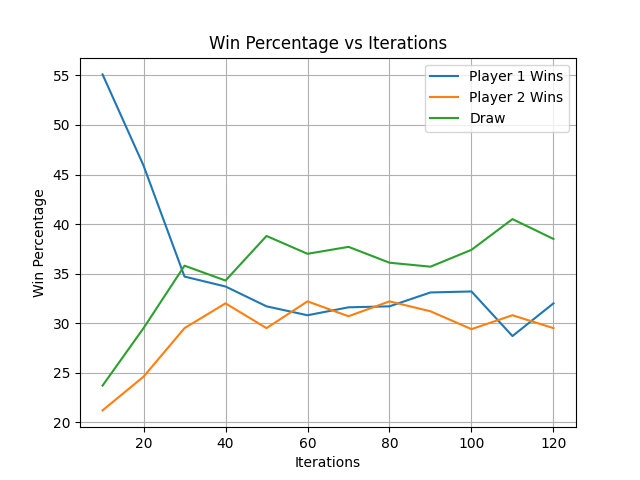
\includegraphics[width=\textwidth]{./MCTS/reward_beta.png}
%         \caption{Reward vs Beta}
%     \end{minipage}
%     \hfill
%     \begin{minipage}[b]{0.45\textwidth}
%         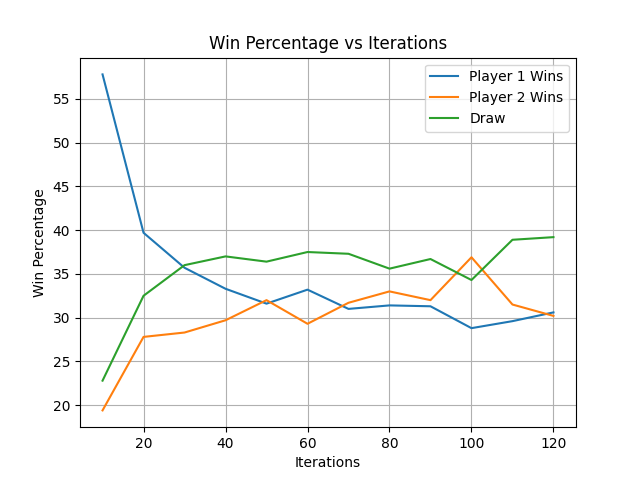
\includegraphics[width=\textwidth]{./MCTS/reward_reward.png}
%         \caption{Reward vs Reward}
%     \end{minipage}
%     \vfill
%     \begin{minipage}[b]{0.45\textwidth}
%         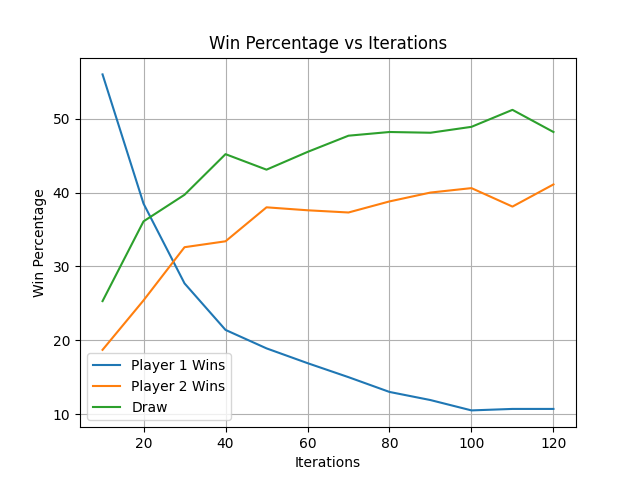
\includegraphics[width=\textwidth]{./MCTS/reward_UCT.png}
%         \caption{Reward vs UCT}
%     \end{minipage}
%     \hfill
%     \begin{minipage}[b]{0.45\textwidth}
%         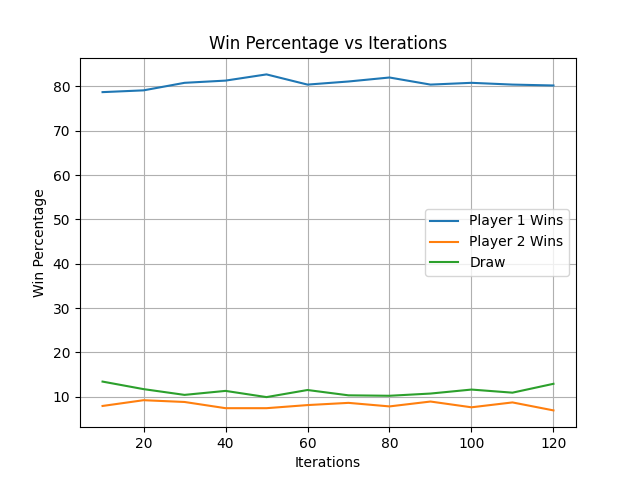
\includegraphics[width=\textwidth]{./MCTS/reward_visited.png}
%         \caption{Reward vs Visited}
%     \end{minipage}
%     \caption{Results of different algorithms on Tic-Tac-Toe}
%     \label{tictactoe}
% \end{figure}
\section{Algorithm Variations}
In this part, we will introduce more algorithms based on the UCB/UCT algorithm.\\
\subsection{Bandit Algorithm}
The definitions we used are as follows:
\begin{itemize}
    \item \(X_{d',n_{d'}}\): The reward received at node \(d'\) after \(n_{d'}\) visits.
    \item \(n_d\): The number of times the node of depth \(d\) in the optimal branch is reached.
    \item \(n\): The first instant when the optimal leaf is reached.
    \item \(D\): The depth of the tree.
    \item \(s\): A constant used in the confidence sequence.
    \item \[B_{i,p,n_i}=^\text{def}X_{i,n_i}+\sqrt{\frac{2\log(p)}{n_i}}\]
\end{itemize}
The pseudeo Code for bandit algorithm is as follows:
\begin{algorithm}[H]
    \caption{Bandit Algorithm}
    \begin{algorithmic}[1]
        \For {$n\ge 1$} 
            \State Run $n-$th trajectory from the root to leaf
            \State set current node $i_0$ to root
            \For {$d=1\cdots D$} 
                \State Select node $i_d$ as the children $j$ of node $i_{d-1}$ that maximizes $B_{j,n_{i_{d-1}},n_j}$
            \EndFor
        \EndFor
    \end{algorithmic}
\end{algorithm}
Coquelin and Munos propose flat UCB which effectively treats the leaves of the search tree as a single multiarmed bandit problem.\cite{coquelin2007bandit} This is distinct from flat Monte Carlo search, in which the actions for a given state are uniformly sampled and no tree is built. Coquelin and Munos demonstrate that flat UCB retains the adaptivity of standard UCT while improving its regret
bounds in certain worst cases where UCT is overly optimistic.\\
Intuitionlly, UCT may spend many time exploring an area that there is no best reward. Let's provide an example: the Monte Carlo tree has $m$ stages, while the $i$-th stage has a decision to get a reward of $\frac{m-(i+1)}{m}$ directly, while in the $m$th stage, you could get a reward of $1$. However, since the UCT algorithm will tend to visit the first stage with a reward of $\frac{m-1}{m}$, it will cost the UCT algorithm many times to explore the last stage whose reward is 1. (It will take UCT $O(\exp(\exp m))$ time).\\
We now establish a lower bound on the number of times suboptimal rewards are received before getting the optimal 1 reward for the first time. Write \(n\) the first instant when the optimal leaf is reached. Write \(n_d\) the number of times the node (also written \(d\) making a slight abuse of notation) of depth \(d\) in the optimal branch is reached. Thus \(n = n_0\) and \(n_D = 1\). At depth \(D - 1\), we have \(n_{D-1} = 2\) (since action 2 has been chosen once in node \(D - 1\)).\\
We consider both the logarithmic confidence sequence used in (1) and the square root sequence in (2). Let us start with the square root confidence sequence (2). At depth \(d - 1\), since the optimal branch is followed by the \(n\)-th trajectory, we have (writing \(d'\) the node resulting from action 2 in the node \(d - 1\)):
\[
X_{d',n_{d'}} + \frac{s\sqrt{n_{d-1}}}{n_{d'}} \leq X_{d,n_d} + \frac{s\sqrt{n_{d-1}}}{n_d}.
\]
But \(X_{d',n_{d'}} = \frac{D - d}{D}\) and \(X_{d,n_d} \leq \frac{D - (d + 1)}{D}\) since the 1 reward has not been received before. We deduce that
\[
\frac{1}{D} \leq \frac{s\sqrt{n_{d-1}}}{n_d}.
\]
Thus for the square root confidence sequence, we have \(n_{d-1} \geq \frac{n_d^2}{D^4}\). Now, by induction,
\[
n \geq \frac{n_1^2}{D^4} \geq \frac{n_2^2}{2D^4(1+2)} \geq \frac{n_3^2}{3D^4(1+2+3)} \geq \cdots \geq \frac{n_{D-1}^2}{(D-1)D^{2D(D-1)}}.
\]
Since \(n_{D-1} = 2\), we obtain \(n \geq \frac{2^{2D-1}}{D^{2D(D-1)}}\). This is a double exponential dependency with respect to \(D\). For example, for \(D = 20\), we have \(n \geq 10^{156837}\). Consequently, the regret is also \(\Omega(\exp(\exp(D)))\).\\
Now, the usual logarithmic confidence sequence defined by (1) yields an even worse lower bound on the regret since we may show similarly that \(n_{d-1} \geq \exp(n_d/(2D^2))\) thus
\[
n \geq \exp(\exp(\cdots \exp(2) \cdots)) \quad (\text{composition of } D - 1 \text{ exponential functions}).
\]
Thus, although UCT algorithm has asymptotically regret \(O(\log(n))\) in \(n\), (or \(O(\sqrt{n})\) for the square root sequence), the transitory regret is \(\Omega(\exp(\exp(\cdots \exp(2) \cdots)))\) (or \(\Omega(\exp(\exp(D)))\) in the square root sequence).\\
The reason for this bad behavior is that the algorithm is too optimistic (it does not explore enough and may take a very long time to discover good branches that looked initially bad) since the bounds (1) and (2) are not true upper bounds.\\

\bibliographystyle{plain}
\bibliography{reference}
\end{document}
